\documentclass[letterpaper, 11pt]{extarticle}

\input{preamble}
\input{format}
\input{commands}

% Listings style for code
\lstset{
    language=Python,
    basicstyle=\ttfamily\small,
    keywordstyle=\color{blue},
    commentstyle=\color{gray}\itshape,
    stringstyle=\color{red},
    showstringspaces=false,
    numbers=left,
    numberstyle=\tiny\color{gray},
    numbersep=8pt,
    breaklines=true,
    frame=single,
    backgroundcolor=\color{gray!5},
}

\begin{document}

\begin{Large}
    \textsf{\textbf{CS361 - HW3}}
\end{Large}

\vspace{1ex}

\textsf{\textbf{Student:}} \text{Shrey Poshiya}\\

Github Link: \href{https://github.com/sposhiy33/CS361HW}{https://github.com/sposhiy33/CS361HW}

\vspace{2ex}


% Problem 1 - Min-heap: at least k numbers smaller than x
\begin{problem}{}{problem-1}
    You are given a min-heap $H$ containing $n$ numbers, an integer $k$, and a number $x$. Design an algorithm that determines whether $H$ contains at least $k$ numbers smaller than $x$, and runs in $O(k)$ time. Your answer must not depend on $n$.
\end{problem}

\vspace{1ex}
\noindent\textbf{Implementation:}
\lstinputlisting[language=Python,caption={Problem 1 (\texttt{Problem1/problem1.py})}]{../HW3/Problem1/problem1.py}

\textbf{Note}: the implementaton of the Min-Heap can be found in the github under the following directory: \texttt{HW3/Problem1}


% Problem 2 - Determine if undirected graph is a tree
\begin{problem}{}{problem-2}
    Suppose you are given an undirected simple graph $G(V, E)$. Design an efficient algorithm to determine if the given graph is a tree or not. Note that you should also discuss how you want the input graph to be represented, e.g., an adjacency list or an adjacency matrix.
\end{problem}

\vspace{1ex}
\noindent\textbf{Implementation:}
\lstinputlisting[language=Python,caption={Problem 2 (\texttt{Problem2/problem2.py})}]{../HW3/Problem2/problem2.py}

\vspace{1ex}
\noindent\textbf{Output:}
\lstinputlisting[language={},caption={Problem 2 output (\texttt{Problem2/problem2.out})}]{../HW3/Problem2/problem2.out}

\vspace{1ex}
\noindent\textbf{Notes:}

To see the specific implementation of the graph, see the following file: \texttt{HW3/Problem2/graph.py}. I opted to use a \text{list representation} for the graph as we are not explicity working with dense graphs, in which case the memory usage of the list and matrix representations would be equiavalent with the matrix having the added benfit of $O(1)$ look up time for edges. But since I am only performing a traversal, I do not need to lookup specific edges; therefore, I cannot utulize the fast lookup time. 

Furthermore, my algorithm involves comparing a nodes entire adjecency set with the visited list. Since the list representation inherently stores the adjacency set, a list representation is the obvious choice (with a matrix representation, I would have to construct this set using extra operations)

% Problem 3 - Rotting Oranges (LeetCode)
\begin{problem}{}{problem-3}
    Solve the Rotting Oranges problem and write the algorithm for your answer. Your solution must pass all test cases, and you must attach a screenshot of your accepted submission.
\end{problem}

\vspace{1ex}
\noindent\textbf{Implementation:}
\lstinputlisting[language=Python,caption={Problem 3 (\texttt{Problem3/problem3.py})}]{../HW3/Problem3/problem3.py}

\vspace{1ex}
\noindent\textbf{Output:}
\lstinputlisting[language={},caption={Problem 3 output (\texttt{Problem3/problem3.out})}]{../HW3/Problem3/problem3.out}

\vspace{1ex}
\noindent\textbf{LeetCode Submission:}

Submission Link: \href{https://leetcode.com/problems/rotting-oranges/submissions/1988162220}{https://leetcode.com/problems/rotting-oranges/submissions/1988162220}

\begin{center}
    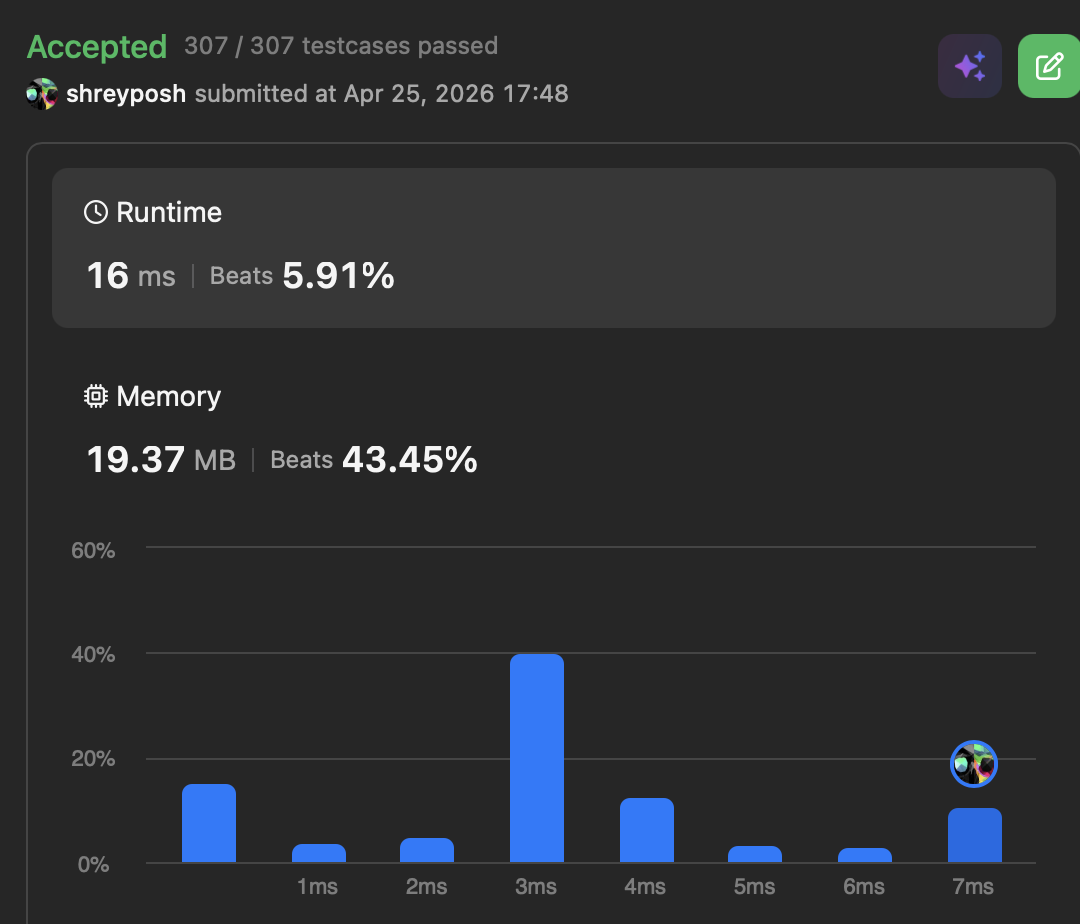
\includegraphics[width=\linewidth]{assets_HW3/RottingOrangesSubmission.png}
\end{center}


% Problem 4 - BFS and DFS Implementation and analysis
\begin{problem}{}{problem-4}
    BFS and DFS Implementation and analysis.
\end{problem}

\vspace{1ex}
\noindent\textbf{Implementation:}
\lstinputlisting[language=Python,caption={Problem 4 (\texttt{Problem4/problem4.py})}]{../HW3/Problem4/problem4.py}

\vspace{1ex}
\noindent\textbf{Output:}
\lstinputlisting[language={},caption={Problem 4 output (\texttt{Problem4/problem4.out})}]{../HW3/Problem4/problem4.out}

\vspace{1ex}
\noindent\textbf{Traversal comparison (visited order until target is found):}
\begin{center}
\begin{tabular}{|c|l|l|c|}
\hline
\textbf{Graph} & \textbf{Variant} & \textbf{Visited order} & \textbf{Length} \\
\hline
(a) & BFS list   & 0, 3, 2, 7 & 4 \\
(a) & BFS matrix & 0, 2, 3, 7 & 4 \\
(a) & DFS list   & 0, 8, 10, 7 & 4 \\
(a) & DFS matrix & 0, 8, 10, 7 & 4 \\
\hline
(b) & BFS list   & A, B, C, D, G, E, H, L, N, K, F, I, O & 13 \\
(b) & BFS matrix & A, B, C, D, G, E, H, K, L, N, F, I, O & 13 \\
(b) & DFS list   & A, C, D, E, K, F, M, O               & 8 \\
(b) & DFS matrix & A, C, D, E, K, L, F, M, O            & 9 \\
\hline
\end{tabular}
\end{center}

\vspace{1ex}
\noindent\textbf{Heatmap (BFS vs DFS, list vs matrix; avg of 5 runs):}
\begin{center}
    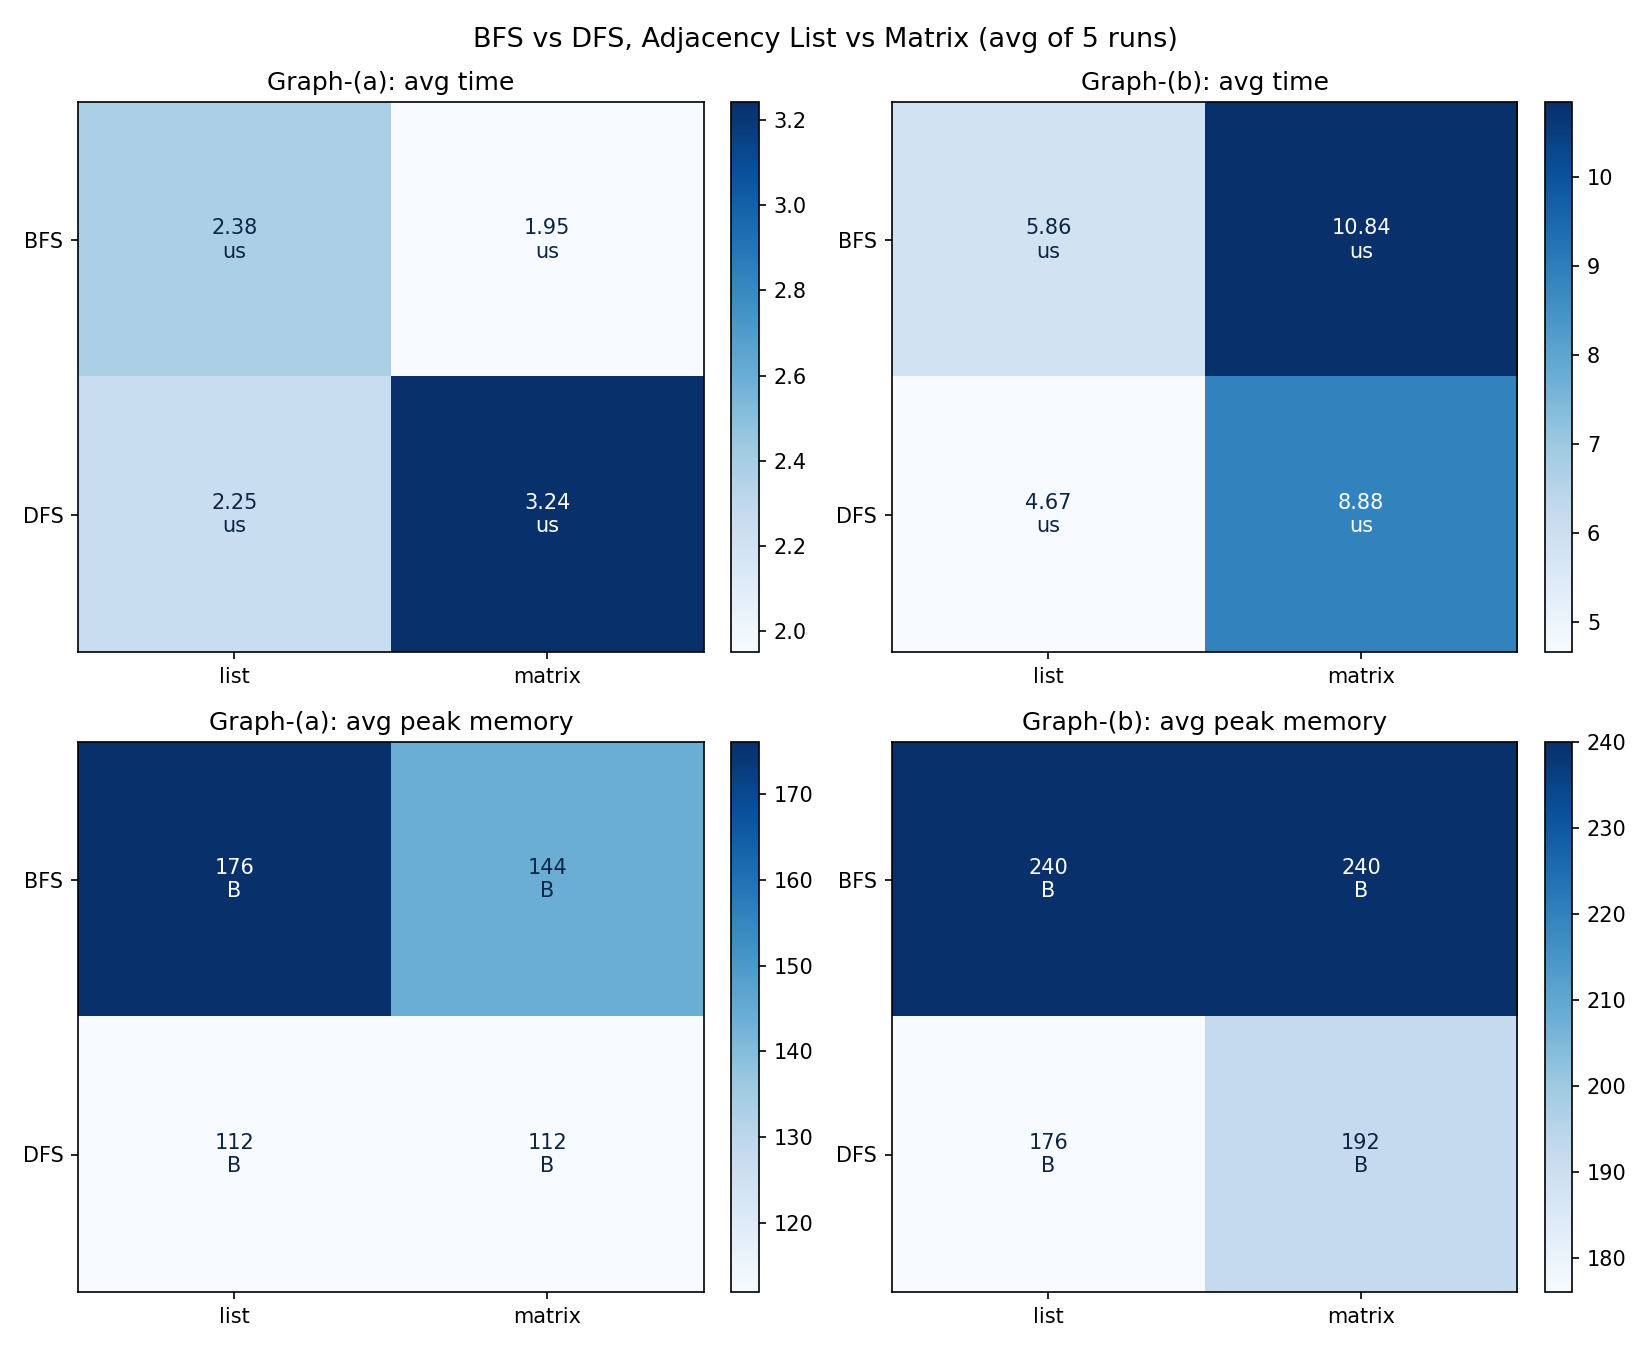
\includegraphics[width=\linewidth]{assets_HW3/problem4_heatmap.png}
\end{center}

\vspace{1ex}
\noindent\textbf{Notes:}

See \texttt{HW3/Problem4} for graph representation code, analysis code (time and memory analysis), and plotting code for the above heatmap. Only the main traversal algorithms are provided in the listing above.

\textit{Graph A}: We see DFS ends up requiring more execution time than BFS. While the traversal counts (not the paths) are all the same, it is likely that DFS algorithm uses more operations throughout its runtime. Overall there is not as much variance between execution times due to the small size of the graph. Surprisngly, each algorithm and graph representation variant ends up have the same traversal count (this is explained later). 

The max memory usage shows that BFS list representation has the largest memaory footprint out of the 4 variants. Since the traversal counts are the same, the visited arrays are all of the same size. This means that the discrepency in memory footprint must come from the queue/stack of the traversal algorithms.

Note: The peak memory metric provides insight into the peak size of the function call, which mainly correlates to peak size of the queue or stack in BFS and DFS respectively and the visited array (my implementation does not account for the memory footprint of the graph objects). 

\textit{Graph B}: Here we see a clear execution time increase when using a matrix representation as opposed to a list representation. This means that the time it takes to retrive all neighbors from the matrix for a given node becomes a bottleneck in the traversal algorithm. In the list representation, the specific neighbor identities for each node are inherently part of the data structure, requiring less operations than the matrix. A larger graph, shows this discrepancy more clearly as compared to the smaller graph A. The peak memory sizes correlate to the size of the visited node list (see above). This means that the queue/stack of the traversal does not have as much impact, meaning that it pretty small compared to the visited list. This goes to show that the size of queue/stack data structure in the traversal algorithm does not necessarily scale with graph size. Overall BFS has a larger memory footprint, most likely a result of the BFS traversals being longer.


\textit{Traversal Paths}: It is obvious to see differences in traversal paths between DFS and BFS, but it is less obvious when comparing list vs matrix representations. The core fact underlying the difference in traversals between these two data structures is: $(1)$ the matrix traverses over neighbors in the order of row/col order (ascending for my BFS implementation and descending for my DFS implementation) while $(2)$ the list representation traverses over neighbors in the order that they were inserted (see analysis.py for this). Surprinsgly, despite the difference in traversal paths, we that the graph A traversals end up being the same length of $4$.

\end{document}
